\begin{frame}
  \begin{enumerate}
    \item
      Use the interactive decision procedure to check if object is invariant
      confluent.
    \pause\item
      If it is, deploy it with weak consistency.
    \pause\item
      If it's not, then...? \pause deploy with strong consistency?
  \end{enumerate}
\end{frame}

\newcommand{\dy}{0.2}
\begin{frame}
  \begin{center}
    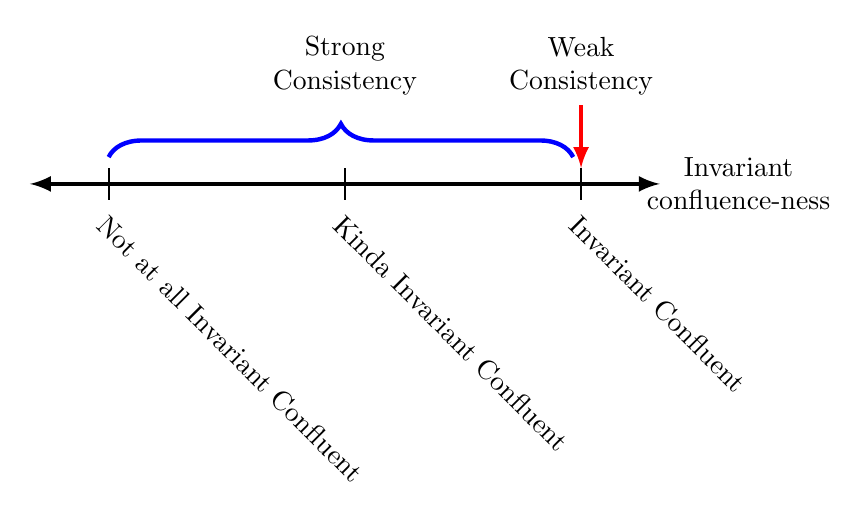
\begin{tikzpicture}
      \draw[ultra thick, latex-latex] (0, 0) to (8, 0);
      \draw[thick] (1, -\dy) to (1, \dy);
      \draw[thick] (4, -\dy) to (4, \dy);
      \draw[thick] (7, -\dy) to (7, \dy);
      \node[align=center] at (9, 0) {Invariant\\confluence-ness};
      \pause
      \node[rotate=-45, anchor=north west] at (7, -\dy) {Invariant Confluent};
      \pause
      \node[rotate=-45, anchor=north west] at (4, -\dy) {Kinda Invariant Confluent};
      \pause
      \node[rotate=-45, anchor=north west] at (1, -\dy) {Not at all Invariant Confluent};

      \pause
      \draw[ultra thick, -latex, red] (7, 1) to (7, \dy);
      \node[align=center, fill=white] at (7, 1.5) {Weak\\Consistency};

      \pause
      \draw[decorate, decoration={brace, amplitude=12pt, raise=4pt},
            ultra thick, blue] (1, \dy) to (6.9, \dy);
      \node[align=center] at (4, 1.5) {Strong\\Consistency};
    \end{tikzpicture}
  \end{center}
\end{frame}

\begin{frame}
  \begin{center}
    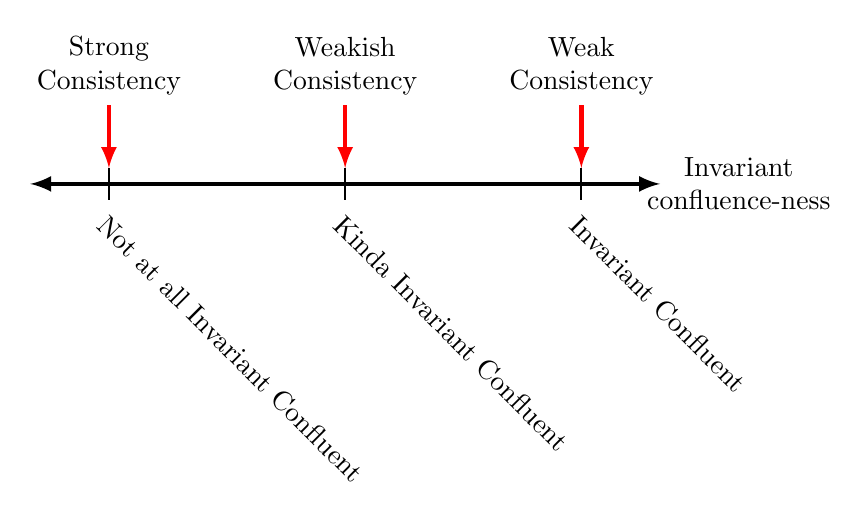
\begin{tikzpicture}
      \draw[ultra thick, latex-latex] (0, 0) to (8, 0);
      \draw[thick] (1, -\dy) to (1, \dy);
      \draw[thick] (4, -\dy) to (4, \dy);
      \draw[thick] (7, -\dy) to (7, \dy);
      \node[align=center] at (9, 0) {Invariant\\confluence-ness};
      \node[rotate=-45, anchor=north west] at (7, -\dy) {Invariant Confluent};
      \node[rotate=-45, anchor=north west] at (4, -\dy) {Kinda Invariant Confluent};
      \node[rotate=-45, anchor=north west] at (1, -\dy) {Not at all Invariant Confluent};

      \draw[ultra thick, -latex, red] (7, 1) to (7, \dy);
      \node[align=center, fill=white] at (7, 1.5) {Weak\\Consistency};
      \draw[ultra thick, -latex, red] (4, 1) to (4, \dy);
      \node[align=center, fill=white] at (4, 1.5) {Weakish\\Consistency};
      \draw[ultra thick, -latex, red] (1, 1) to (1, \dy);
      \node[align=center, fill=white] at (1, 1.5) {Strong\\Consistency};
    \end{tikzpicture}
  \end{center}
\end{frame}

\begin{frame}
  \begin{center}
    \Large
    \defword{Segmented invariant confluence}: divide state space into segments;
    operate with weak consistency within segments and strong consistency across
    segments.
  \end{center}
\end{frame}

\begin{frame}
  A \defword{segmentation} $\Sigma = (I_1, T_1), \ldots, (I_n, T_n)$ is a
  sequence (not a set) of $n$ segments $(I_i, T_i)$.
  \pause
  $O$ is \defword{segmented \invariantconfluent{}} with respect to $s_0$, $T$,
  $I$, and $\Sigma$, abbreviated \defword{\sTISconfluent}, if the following
  conditions hold:
  \begin{itemize}
    \pause\item
      The start state satisfies the invariant (i.e. $I(s_0)$).

    \pause\item
      $I$ is covered by the invariants in $\Sigma$.

    \pause\item
      $O$ is \invariantconfluent{} within each segment. That is, for every $(I_i,
      T_i) \in \Sigma$ and for every state $s \in I_i$, $O$ is
      \sticonfluent{s}{T_i}{I_i}.
  \end{itemize}
\end{frame}

{
\newcommand{\xmin}{-2}
\newcommand{\xmax}{2}
\newcommand{\ymin}{-2}
\newcommand{\ymax}{2}

% Axes.
\newcommand{\xyaxes}{
  \draw[] (\xmin.5, 0) to (\xmax.5, 0);
  \draw[] (0, \ymin.5) to (0, \ymax.5);
  \node at (\xmax + 1, 0) {$x$};
  \node at (0, \ymax + 1) {$y$};
}

% Quadrant 1.
\newcommand{\quadi}[5]{{
  \newcommand{\argstyle}{#1}
  \newcommand{\argxmin}{#2}
  \newcommand{\argxmax}{#3}
  \newcommand{\argymin}{#4}
  \newcommand{\argymax}{#5}
  \foreach \x in {0, ..., \argxmax} {
    \foreach \y in {0, ..., \argymax} {
      \node[\argstyle] (\x-\y) at (\x, \y) {};
    }
  }
}}

% Quadrant 2.
\newcommand{\quadii}[5]{{
  \newcommand{\argstyle}{#1}
  \newcommand{\argxmin}{#2}
  \newcommand{\argxmax}{#3}
  \newcommand{\argymin}{#4}
  \newcommand{\argymax}{#5}
  \foreach \x in {\argxmin, ..., 0} {
    \foreach \y in {0, ..., \argymax} {
      \node[\argstyle] (\x-\y) at (\x, \y) {};
    }
  }
}}

% Quadrant 3.
\newcommand{\quadiii}[5]{{
  \newcommand{\argstyle}{#1}
  \newcommand{\argxmin}{#2}
  \newcommand{\argxmax}{#3}
  \newcommand{\argymin}{#4}
  \newcommand{\argymax}{#5}
  \foreach \x in {\argxmin, ..., 0} {
    \foreach \y in {\argymin, ..., 0} {
      \node[\argstyle] (\x-\y) at (\x, \y) {};
    }
  }
}}

% Quadrant 4.
\newcommand{\quadiv}[5]{{
  \newcommand{\argstyle}{#1}
  \newcommand{\argxmin}{#2}
  \newcommand{\argxmax}{#3}
  \newcommand{\argymin}{#4}
  \newcommand{\argymax}{#5}
  \foreach \x in {0, ..., \argxmax} {
    \foreach \y in {\argymin, ..., 0} {
      \node[\argstyle] (\x-\y) at (\x, \y) {};
    }
  }
}}

% State labels.
\newcommand{\statelabels}{
  \node[statelabel] at (0, 0) {$s_0$};
  \node[statelabel] at (-1, 1) {$s_1$};
  \node[statelabel] at (1, -1) {$s_2$};
  \node[statelabel] at (1, 1) {$s_3$};
}

\tikzstyle{point}=[shape=circle, fill=flatgray, inner sep=3pt]
\tikzstyle{inv}=[line width=0.75pt, draw=black]
\tikzstyle{pointinv}=[point, inv]
\tikzstyle{invregion}=[rounded corners, fill=flatgreen!50, draw=none]
\tikzstyle{reachableregion}=[rounded corners, fill=flatblue!50, draw=none]
\tikzstyle{statelabel}=[anchor=south west, inner sep=1pt]

\begin{frame}
  \begin{columns}
    \begin{column}{0.5\textwidth}
      \centering
      \begin{tikzpicture}[scale=1]
        \begin{scope}
          \clip (\xmin.5, \ymax.5) rectangle (\xmax.5, \ymin.5);
          \draw[invregion] (\xmin.9, \ymax.9) rectangle (0.5, -0.5);
          \draw[invregion] (-0.5, 0.5) rectangle (\xmax.9, \ymin.9);
          \draw (0.5, 0.5) to (0.5, \ymax.5);
          \draw (0.5, 0.5) to (\xmax.5, 0.5);
          \draw (-0.5, -0.5) to (-0.5, \ymin.5);
          \draw (-0.5, -0.5) to (\xmin.5, -0.5);
        \end{scope}

        \xyaxes{}
        \quadi{point}{\xmin}{\xmax}{\ymin}{\ymax}
        \quadiii{point}{\xmin}{\xmax}{\ymin}{\ymax}
        \quadii{pointinv}{\xmin}{\xmax}{\ymin}{\ymax}
        \quadiv{pointinv}{\xmin}{\xmax}{\ymin}{\ymax}
      \end{tikzpicture}

      {\Huge Invariant}
    \end{column}
    \begin{column}{0.5\textwidth}
      \pause
      \centering
      \begin{tikzpicture}[scale=1]
        \begin{scope}
          \clip (-3, 3) rectangle (\xmax.5, \ymin.5);
          \draw[reachableregion, draw=black] (-2.5, 2.5) rectangle (\xmax.9, \ymin.9);
        \end{scope}

        \xyaxes{}
        \quadi{pointinv}{\xmin}{\xmax}{\ymin}{\ymax}
        \quadiii{pointinv}{\xmin}{\xmax}{\ymin}{\ymax}
        \quadii{pointinv}{\xmin}{\xmax}{\ymin}{\ymax}
        \quadiv{pointinv}{\xmin}{\xmax}{\ymin}{\ymax}
      \end{tikzpicture}

      {\Huge Reachable}
    \end{column}
  \end{columns}
\end{frame}
}

{
\tikzstyle{point}=[shape=circle, fill=flatgray, inner sep=2pt, draw=black]
\tikzstyle{region}=[draw=none]
\tikzstyle{region1}=[region, fill=flatred!50]
\tikzstyle{region2}=[region, fill=flatgreen!50]
\tikzstyle{region3}=[region, fill=flatblue!50]
\tikzstyle{region4}=[region, fill=flatpurple!50]

\newcommand{\pointgrid}[4]{{
  \newcommand{\argxmin}{#1}
  \newcommand{\argxmax}{#2}
  \newcommand{\argymin}{#3}
  \newcommand{\argymax}{#4}

  \draw[] (\argxmin, 0) to (\argxmax, 0);
  \draw[] (0, \argymin) to (0, \argymax);
  \foreach \x in {\argxmin, ..., \argxmax} {
    \foreach \y in {\argymin, ..., \argymax} {
      \node[point] (\x-\y) at (\x, \y) {};
    }
  }
}}

\newcommand{\subfigwidth}{0.24\columnwidth}
\newcommand{\subfighspace}{0.3cm}
\newcommand{\tikzhspace}{0.4cm}
\newcommand{\tikzscale}{0.75}
\newcommand{\xmin}{-2}
\newcommand{\xmax}{2}
\newcommand{\ymin}{-2}
\newcommand{\ymax}{2}

\begin{frame}
  \begin{center}
    \begin{tikzpicture}[scale=\tikzscale]
      \draw[white] (-3, -3) to (3, 3);
      \draw[region1] (\xmin.5, \ymax.5) rectangle (-0.5, 0.5);
      \draw (-0.5, 0.5) to (\xmin.5, 0.5);
      \draw (-0.5, 0.5) to (-0.5, \ymax.5);
      \pointgrid{\xmin}{\xmax}{\ymin}{\ymax}
    \end{tikzpicture}%
    \hspace{0.1in}%
    \begin{tikzpicture}[scale=\tikzscale]
      \draw[white] (-3, -3) to (3, 3);
      \draw[region2] (-0.5, 0.5) rectangle (\xmax.5, \ymin.5);
      \draw (-0.5, 0.5) to (\xmax.5, 0.5);
      \draw (-0.5, 0.5) to (-0.5, \ymin.5);
      \pointgrid{\xmin}{\xmax}{\ymin}{\ymax}
    \end{tikzpicture}

    \begin{tikzpicture}[scale=\tikzscale]
      \draw[white] (-3, -3) to (3, 3);
      \draw[region3] (-0.5, \ymax.5) rectangle (0.5, \ymin.5);
      \draw (-0.5, \ymax.5) to (-0.5, \ymin.5);
      \draw (0.5, \ymax.5) to (0.5, \ymin.5);
      \pointgrid{\xmin}{\xmax}{\ymin}{\ymax}
    \end{tikzpicture}%
    \hspace{0.1in}%
    \begin{tikzpicture}[scale=\tikzscale]
      \draw[white] (-3, -3) to (3, 3);
      \draw[region4] (\xmin.5, 0.5) rectangle (\xmax.5, -0.5);
      \draw (\xmax.5, -0.5) to (\xmin.5, -0.5);
      \draw (\xmax.5, 0.5) to (\xmin.5, 0.5);
      \pointgrid{\xmin}{\xmax}{\ymin}{\ymax}
    \end{tikzpicture}
  \end{center}
\end{frame}
}
